\documentclass[dissertation.tex]{subfiles}

\begin{document}

The compiler is comprised of a number of stages and substages, as shown in Figure \ref{fig:compiler-layout}:

\begin{figure}[h]
    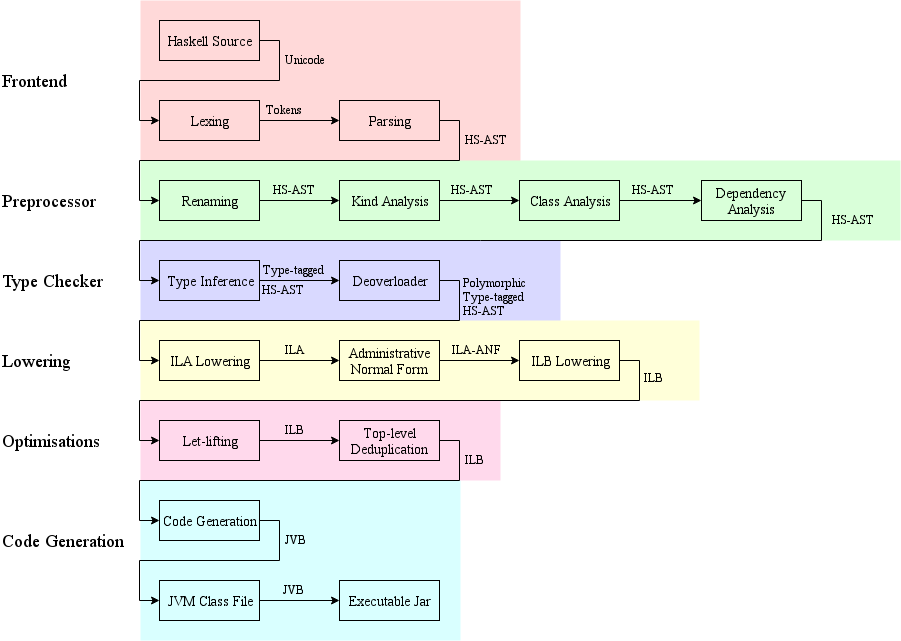
\includegraphics[width=\textwidth]{figures/compiler_layout.png}
    \caption{}
    \label{fig:compiler-layout}
\end{figure}

A brief overview of each stage is given here for a `big picture' view of the compiler, followed by more detailed
descriptions below.

\begin{description}
\item[Frontend]
{
    \hfill

    The frontend consists of standard lexing and parsing from Haskell source code into an Abstract Syntax Tree
    (AST). A modified version of an existing library (haskell-src\footnote{https://github.com/hnefatl/haskell-src})
    is used.

}
\item[Preprocessing]
{
    \hfill
    \begin{itemize}
    \item
    {

        The renamer renames each variable so that later stages can assume each variable name is unique:
        this reduces complexity by removing the possibility of variable shadowing (eg.\ \haskell{let x = 1 in let x = 2 in x}).

    }
    \item
    {

        Kind and Class analysis both simply extract useful information about the declarations in the source so that
        stages of the type checker are simpler.

    }
    \item
    {

        Dependency analysis computes a partial order on the source declarations so that the typechecker can process
        them in a valid order.

    }
    \end{itemize}
}
\item[Type Checker]
{
    \hfill
    \begin{itemize}
    \item
    {

        The type inference stage infers polymorphic overloaded types for each symbol, checks them against any
        user-provided type signatures, and alters the AST so that each expression is tagged with its type.

    }
    \item
    {

        Deoverloading converts polymorphic overloaded types to polymorphic types similar to those of System F, and
        alters the AST to implement typeclasses using dictionary-passing.

    }
    \end{itemize}
}
\item[Lowering]
{
    \hfill

    The lowering stage transforms the Haskell source AST into Intermediate Language A (ILA), then rearranges that
    tree into Administrative Normal Form (ILA-ANF), before finally transforming it into Intermediate Language B
    (ILB).

}
\item[Optimisations]
{
    \hfill

    Optimisations transform the intermediate languages into more efficient forms while preserving their semantics.

    \todo[inline]{At time of writing these are done on ILB, might change to ILAANF so should update this accordingly.}
    \todo[inline]{If any more optimisations are implemented, update the diagram and here.}

}
\item[Code Generation]
{
    \hfill

    ILB is transformed into Java Bytecode (JVB), and a modified version of an existing library
    (hs-java\footnote{https://github.com/hnefatl/hs-java}) is used to convert a logical representation of the
    bytecode into a set of class files, which are then packaged into an executable Jar file.

}
\end{description}


\section{Implementation Details}
{
    \subsection{Frontend}
    {

        Lexing and parsing of Haskell source is performed using the
        \monospace{haskell-src}\footnote{https://hackage.haskell.org/package/haskell-src} library, which I have modified
        to provide some additional desirable features:

        \begin{itemize}
        \item
        {
            Lexing and parsing declarations for built-in constructors like list and tuple definitions (eg.\
            \haskell{data [] a = [] | a:[a]}).
        }
        \item
        {
            Parsing data declarations without any constructors (eg.\ \haskell{data Int})\footnote{Declarations of this
            form are invalid in the original Haskell 1998 syntax, but valid in Haskell 2010: see
            https://wiki.haskell.org/Empty\_type}. This is a valuable way of introducing built-in types.
        }
        \item
        {
            Adding \haskell{Hashable} and \haskell{Ord} typeclass instances to the syntax AST, so that syntax trees can
            be stored in associative containers.
        }
        \end{itemize}

        The syntax supported is a strict superset of Haskell 1998 and a strict subset of Haskell 2010, but my compiler
        does not have support for all of the features implied by the scope of the syntax. For example, multi-parameter
        typeclasses are parsed correctly as a feature of Haskell 2010 but get rejected by the deoverloading stage.

        \begin{figure}[h]
            \begin{haskellfigure}
            class Convertable a b where
                convert :: a -> b
            instance Convertable Bool Int where
                convert True = 1
                convert False = 0
            \end{haskellfigure}
            \caption{An example of a multi-parameter typeclass}
        \end{figure}

    }
    \subsection{Preprocessor}
    {
        \subsubsection{Renaming}
        {

            Haskell allows for multiple variables to share the same name within different scopes, which can increase the
            complexity of later stages in the pipeline. For example, when typechecking the following code we might
            conflate the two uses of \haskell{x}, and erroneously infer that they have the same type. A similar problem
            arises with variable shadowing, when the scopes overlap. The problem also applies to any type variables
            present in the source -- the type variable \haskell{a} is distinct between the two type signatures:

            \begin{haskellfigure}
            id :: a -> a
            id x = x

            const :: a -> b -> a
            const x _ = x
            \end{haskellfigure}

            Additionally, variables and type variables are in different namespaces: the same token can refer to a
            variable and a type variable, even within the same scope. The following code is perfectly valid (but loops
            forever), despite the same name being used for a type variable and a variable:

            \begin{haskellfigure}
            x :: x
            x = x
            \end{haskellfigure}

            To eliminate the potential for subtle bugs stemming from this feature, the renamer pass gives each distinct
            variable/type variable in the source a unique name (in the above example, the variable \haskell{x} might be
            renamed to \haskell{v0} and the type variable renamed to \haskell{tv0}, provided those names haven't been
            already used).
            
            Unique variable/type variable names are generated by prefixing the current value of an incrementing counter
            with either \haskell{v} for variable names or \haskell{tv} for type variable names. The renamer traverses
            the syntax tree maintaining a mapping from a syntactic variable/type variable name to an associated stack of
            unique semantic variable names (in Haskell, a \haskell{Map VariableName [UniqueVariableName]}):

            \begin{itemize}
            \item When processing the binding site of a new syntactic variable (eg.\ a let binding, a lambda argument, a
            pattern match...), a fresh semantic name is generated and pushed onto the stack associated with the
            syntactic variable.
            \item Whenever we leave the scope of a syntactic variable, we pop the top semantic name from the associated
            stack.
            \item When processing a use site of a syntactic variable, we replace it with the current top of the
            associated stack.
            \end{itemize}

            An analogously constructed mapping is maintained for type variables, but is kept separate from the variable
            mapping: otherwise the keys can conflict in code such as \haskell{x :: x}.

            Type constants, such as \haskell{Bool} from \haskell{data Bool = False | True} and typeclass names like
            \haskell{Num} from \haskell{class Num a where ...}, are not renamed: these names are already guaranteed to
            be unique by the syntax of Haskell, and renaming them means we need to maintain more mappings and carry more
            state through the compiler as to what they've been renamed to.

        }
        \subsection{Kind/Class Analysis}
        {

            The typechecker and deoverloader require information about the kinds of any type constructors (the `type of
            the type', eg.\ \haskell{Int :: *} and \haskell{Maybe :: * -> *}), and the methods provided by different
            classes. This is tricky to compute during typechecking as those passes traverse the AST in dependency order.
            Instead, we just perform a traversal of the AST early in the pipeline to aggregate the required information.

        }
        \subsection{Dependency Analysis}
        {

            When typechecking, the order of processing declarations matters: we can't infer the type of \haskell{foo =
            bar baz} until we've inferred the types of \haskell{bar} and \haskell{baz}. The dependency analysis stage
            determines the order in which the typechecker should process declarations.

            We compute the sets of free/bound variables/type variables/type constants for each declaration, then
            construct a dependency graph -- each node is a declaration, and there's an edge from \(A\) to \(B\) if any
            of the bound variables/type variables/type constants at \(A\) are free in \(B\). It is important to
            distinguish between variables/type variables and type constants, as otherwise name conflicts could occur (as
            we don't rename type constants). This separation is upheld in the compiler by using different types for
            each, and is represented in the dependency graph below by colouring variables red and constants blue.

            The strongly connected components of the dependency graph correspond to sets of mutually recursive
            declarations, and the partial order between components gives us the order to typecheck each set. For
            example, from the dependency graph in Figure \ref{fig:dependency-graph} we know that: we need to typecheck
            \(d_3\), \(d_4\), and \(d_5\) together as they're contained within the same strongly-connected component so
            are mutually recursive; we have to typecheck \(d_2\) last, after both other components.

            \begin{figure}[h]
            \centering
            \begin{subfigure}[b]{0.45\textwidth}
                \begin{haskellfigure*}{linenos=false}
                data Bool = False | True      #\(d_1\)#
                x = f True                    #\(d_2\)#
                f y = g y                     #\(d_3\)#
                g y = h y                     #\(d_4\)#
                h y = f y                     #\(d_5\)#
                \end{haskellfigure*}
            \end{subfigure}
            \begin{subfigure}[b]{0.5\textwidth}
                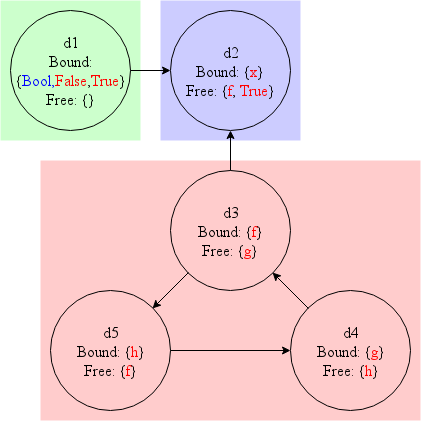
\includegraphics[width=\textwidth]{figures/dependency_graph.png}
            \end{subfigure}
            \caption
            {
                Code labelled with declaration numbers, and the corresponding dependency graph. Variables are
                in red text, type constants in blue. Strongly connected components are highlighted.
            }
            \label{fig:dependency-graph}
            \todo[inline]{Prettier graph: better colours/some other grouping style, and use a more latex-y font.}
            \end{figure}

            Typechecking declarations within the same component can proceed in an arbitrary order, we just need to
            ensure that the all of the type variables for the names bound by the declarations are available while
            processing each individual declaration.

            This process works for languages without ad-hoc overloading, like SML. However, in Haskell there are some
            complications introduced by typeclasses:

            \begin{itemize}
            \item
            {
                Typeclass member variables can be declared multiple times within the same scope. For example:
                
                \begin{haskellfigure}
                class Num a where
                    (+) :: a -> a -> a
                instance Num Int where
                    x + y = ...
                instance Num Float where
                    x + y = ...
                \end{haskellfigure}

                Here the multiple declarations of \haskell{+} don't conflict: this is a valid program. However, the
                following program does have conflicting variables, as \haskell{x} is not a typeclass member and is not
                declared inside an \haskell{instance} declaration:

                \begin{haskellfigure}
                x = True
                x = False
                \end{haskellfigure}

                These declaration conflicts can be expressed as a binary symmetric predicate on declarations, as
                presented in Figure \ref{fig:conflict-grid}, where:

                \begin{itemize}
                \item
                {

                    \monospace{Sym #\(x\)#} and \monospace{Type #\(x\)#} represent top-level declaration and
                    type-signature declarations for a symbol \(x\), like \haskell{#\(x\)# = True} and \haskell{#\(x\)# :: Bool}.

                }
                \item
                {
                    
                    \monospace{ClassSym #\(x\)# #\(c\)#} and \monospace{ClassType #\(x\)# #\(c\)#} represent
                    \monospace{Sym #\(x\)#} and \monospace{Type #\(x\)#} inside the declaration for a class \(c\), like
                    \haskell{class #\(c\)# where { #\(x\)# = True ; #\(x\)# :: Bool }}.

                }
                \item
                {

                    \monospace{InstSym #\(x\)# #\(c\)# #\(t\)#} represents a \monospace{Sym #\(x\)#} inside the
                    declaration for a class instance \(c\;t\), like \haskell{instance #\(c\)# #\(t\)# where { #\(x\)# = True }}.

                }
                \end{itemize}

                \begin{figure}[h]
                \small
                \setlength{\tabcolsep}{2pt}
                \begin{tabular}{ l | c c c c c }
                & \texttt{Sym} \(x_1\) & \texttt{Type} \(x_1\) & \texttt{ClassSym} \(x_1\) \(c_1\) &
                \texttt{ClassType} \(x_1\) \(c_1\) & \texttt{InstSym} \(x_1\) \(c_1\) \(t_1\) \\
                \hline
                \texttt{Sym} \(x_2\) & \(x_1=x_2\) & \texttt{False} & \(x_1=x_2\) & \(x_1=x_2\) & \(x_1=x_2\) \\
                \texttt{Type} \(x_2\) & & \(x_1=x_2\) & \(x_1=x_2\) & \(x_1=x_2\) & \(x_1=x_2\) \\
                \texttt{ClassSym} \(x_2\) \(c_2\) & & & \(x_1=x_2\) & \(x_1=x_2 \wedge c_1 \neq c_2\) & \(x_1=x_2 \wedge c_1 \neq c_2\) \\
                \texttt{ClassType} \(x_2\) \(c_2\) & & & & \(x_1=x_2\) & \(x_1=x_2 \wedge c_1 \neq c_2\) \\
                \texttt{InstSym} \(x_2\) \(c_2\) \(t_2\) & & & & & \makecell{\(x_1=x_2 \wedge (c_1 \neq c_2 \vee t_1=t_2)\)}
                \\
                \end{tabular}
                \caption{The conflict relation: the bottom triangle is omitted as the predicate is symmetric}
                \label{fig:conflict-grid}
                \end{figure}

                Using this table we can see that the multiple declarations for \haskell{+} in the example above are
                \monospace{InstSym (+) Num Int} and \monospace{InstSym (+) Num Float} so do not conflict, while the
                declarations for \haskell{x} above are both \monospace{Sym x} so do conflict.

            }
            \item
            {

                Another complication introduced by typeclasses is that variable declarations such as \haskell{id = \\x
                -> x} are usually treated as being the unique binding definition of \haskell{id}, and any other uses
                within the same level of scope must be free rather than binding (otherwise we have conflicting
                definitions).
                
                However, we treat binding declarations inside \haskell{instance} declarations as actually being free
                uses rather than binding uses, so that the instance declaration forms a dependence on the class
                declaration where the variables are bound, ensuring it is typechecked first.

            }
            \item
            {

                The dependencies generated by this technique are \textit{syntactic}, not \textit{semantic}: this is a
                subtle but very important difference. The use of any ad-hoc overloaded variable generates dependencies
                on the class declaration that introduced the variable, but not the specific instance of the class that
                provides the definition of the variable used.

                \begin{haskellfigure}
                class Foo a where
                    foo :: a -> Bool
                instance Foo Bool where
                    foo x = x
                instance Foo [Bool] where
                    foo xs = all foo xs
                \end{haskellfigure}

                The declaration of \haskell{foo} in \haskell{instance Foo [Bool]} semantically depends on the specific
                overload of \haskell{foo} defined in \haskell{instance Foo Bool}, and yet no dependency will be
                generated between the two instances as neither declaration binds \haskell{foo} (\haskell{foo} is treated
                as being free within the declarations as described above): they will only generate dependencies to
                \haskell{class Foo a} (and to the declaration of \haskell{Bool} and \haskell{all}).

                Computing the semantic dependencies is too complicated to be done in this pass, so the problem is left
                and instead solved during the typechecking stage. A full explanation is given later, but the approach
                used is to defer typechecking instance declarations until a different declaration requires the
                information, and then attempt to typecheck the instance declaration then, in a Just-In-Time manner.

                \todo[inline]{Make sure this is actually explained later}
            }
            \end{itemize}
        }

    }
    \subsection{Type Checker}
    {

        Type inference and checking is the most complex part of the compiler pipeline. The type system implemented is
        intended to be similar to GHC's dialect of Haskell: approximately System \(\text{F}_\omega\) (the
        polymorphically typed lambda calculus with type constructors) along with algebraic data types and type classes
        to provide ad-hoc overloading. The approximation is due to a number of alterations made by the Haskell Report to
        ensure that type inference is decidable, along with the introduction of terms that aren't covered by the pure
        type system eg.\ literals such as \haskell{7} and \haskell{"foo"}. Finally, due to the complexity of the
        implementation there will doubtless be bugs affecting correctness in more complex cases not covered by tests.
        
        This is a subset of the type system used by GHC (System \(\text{F}_\text{C}\)), as that compiler provides
        extensions such as GADTs and type families requiring a more complex type system.

        The full grammar of types as defined in the compiler are explained below:

        \begin{haskellfigure}
        data Kind = KindStar
                  | KindFun Kind Kind
        \end{haskellfigure}

        A \haskell{Kind} is `the type of a type', and is used to describe type constructors: what characterises
        \(\text{Maybe}\) versus \(\text{Maybe}\;\alpha\)?
        
        : while the term \haskell{f} might have the type
        \(\alpha\rightarrow\text{Maybe}\;\alpha\), the type has \textit{kind} \texttt{*}. 

        \todo[inline]{Finish describing kinds and the other type datatypes}

        \todo[inline]{Work out how to use | without the red box in the pdf.}

        \begin{haskellfigure}
        data TypeVariable = TypeVariable TypeVariableName Kind

        data Type = TypeVar TypeVariable
                  | TypeCon TypeConstant
                  | TypeApp Type Type Kind


        data TypePredicate = IsInstance ClassName Type

        data Qualified a = Qualified (Set TypePredicate) a
        type QualifiedType = Qualified Type

        data Quantified a = Quantified (Set TypeVariable) a
        type QuantifiedType = Quantified QualifiedType
        type QuantifiedSimpleType = Quantified Type
        \end{haskellfigure}



        \todo[inline]{Include examples of types demonstrating the features? Examples below might be sufficient. Think an appendix would be best, or should I just include here?}
        \todo[inline]{Include simple BNF grammar for the valid types: can modify the one on the HM wiki page}

        \todo[inline]{Substituion section explaining the basic notation? Used quite a lot in the next few subsubsections}

        \subsubsection{Type Inference}
        {
            \todo[inline]{This whole section needs a lot of attention. The process is complex, maybe need to present the HM rules and their haskell-style variations? Nontrivial}

            % Instantiation of universal types
            % Pass for building substitution and doing tagging, pass for updating tags, pass for checking tags?
            % Patterns
            % Instance typing, with on-demand loading of instances. Refer back to renaming section
            % Mention Outside-In(X) as improvement
            % Mention Hindley-Milner is normally implemented impurely with a graph and updating references when types
            % are resolved. Could have done it that way (maybe should've), but didn't. Compiler is fully pure within the
            % pipeline.

            The implementation is inspired by \cite{THIH}, and proceeds similarly to the Hindley-Milner (HM) type
            inference algorithm presented in \cite{HM-rules}. Following the naming convention using in \cite{THIH}, we
            refer to types such as \(\alpha\rightarrow\alpha\) as `simple types' (`monotypes' in HM), types with
            constraints such as \(\text{Eq}\alpha \Rightarrow \alpha\rightarrow\alpha\rightarrow\text{Bool}\) as
            `overloaded types', and types involving quantifiers such as \(\forall\alpha.\;\text{Monoid }\alpha
            \Rightarrow \alpha\rightarrow\alpha\rightarrow\alpha\) as `polymorphic types' (similar to `polytypes' in HM
            except the quantifiers may wrap an overloaded type or a simple type). It's often helpful to consider simple
            types as the special case of an overloaded type with an empty context (\(\emptyset \Rightarrow t\)).
            
            We process each declaration in dependency order, traversing the AST and tagging each expression with a type
            variable and unifying types together to derive a substitution from type variables to types. Each term in the
            syntax has an associated rule for combining the type variables representing the types of its sub-terms,
            which are computed recursively.

            One departure from the HM algorithm is that Haskell doesn't require \(\Lambda\) terms in the source language
            (explicit `forall' terms that generate \(\forall\) quantifiers on type variables): let-bound variables are
            implicitly polymorphic over all their free type variables, while function parameters are never polymorphic.
            In practice, this means that in Figure \ref{code:polymorphic-let}, \haskell{f :: #\(\forall \alpha.\;\alpha
            \rightarrow a\)#} whereas \haskell{g :: #\(\alpha \rightarrow \alpha\)#}. The difference in semantics
            ensures that type inference remains decidable.
 
            \begin{figure}[h]
            \begin{haskellfigure}
            let f x = x in const (f True) (f 1) :: Bool -- This is fine
            (\\g -> const (g True) (g 1)) (\x -> x)     -- This fails to typecheck
            \end{haskellfigure}
            \caption{}
            \label{code:polymorphic-let}
            \end{figure}
            
            Another major difference from HM is the introduction of typeclasses: whenever we encounter an overloaded
            variable such as \haskell{+}, we split the overloaded type into the constraints \(\{\text{Num }\alpha\}\)
            and the simple type \(\alpha\rightarrow\alpha\rightarrow\alpha\). Unification can be performed as in HM on
            the simple types, but we also maintain a global set of the constraints on type variables that we encounter.
            After unification has completed, we use this set to add the typeclass constraints to the inferred types.

            The final important difference from HM is in the instantiation of polymorphic types: the \([\texttt{Inst}]\)
            rule in HM allows for terms with polymorphic types to be reused at call sites with different argument types,
            but it needs a slight modification to handle type variable constraints introduced by overloaded types:
            
            \begin{figure*}[h]
            \centering
            \begin{subfigure}[t]{0.3\textwidth}
            \begin{displaymath}
            \prftree[r]{\([\text{Inst}]\)}
            {\prfassumption{\Gamma\vdash e : \tau'}}
            {\prfassumption{\tau' \sqsubseteq \tau}}
            {\Gamma\vdash e : \tau}
            \end{displaymath}
            \caption*{The original rule from HM}
            \end{subfigure}
            ~
            \begin{subfigure}[t]{0.6\textwidth}
            \begin{displaymath}
            \prftree[r]{\([\text{Inst}]\)}
            {\prfassumption{\Gamma\stackrel{\Delta}{\vdash} e : C\Rightarrow\tau'}}
            {\prfassumption{\tau' \sqsubseteq \tau}}
            {\prfassumption{\theta = \text{mgu}(\tau, \tau')}}
            {\Gamma\stackrel{\Delta\;\cup\;C\theta}{\vdash} e : C\theta\Rightarrow\tau}
            \end{displaymath}
            \caption*{A modified rule handling type classes. \(\Delta\) is the set of type variable constraints, built up throughout uses of the rules.}
            \end{subfigure}
            \end{figure*}

            \todo[inline]{Bother explaining \(\sqsubseteq\) or just say it means `x is more general than y'? Not exactly going into detail here anyway}
            \todo[inline]{Yeah this is kinda obscure...}

            Here is an example of how the type inference algorithm proceeds on a simple Haskell program:
            \todo[inline]{Want to distinguish as a different section from the above somehow}

            \begin{haskellfigure}
            add1 x = x + 1
            y = add1 2
            \end{haskellfigure}

            As the definition of \haskell{y} depends on the definition of \haskell{add1} we process \haskell{add1}
            first, converting the infix operator into a prefix operator, and producing a type-variable-tagged AST:

            \begin{haskellfigure}
            add1#\(^\alpha\)# x#\(^\beta\)# = (((+)#\(^{\gamma \rightarrow \gamma \rightarrow \gamma}\)#x#\(^\beta\)#)#\(^\delta\)# 1#\(^\epsilon\)#)#\(^\eta\)|
            \end{haskellfigure}

            We know the type of \haskell{+} is \(\forall\omega.\;\text{Num }\omega \Rightarrow
            \omega\rightarrow\omega\rightarrow\omega\) from the definition of \haskell{+} within the typeclass
            \haskell{Num}, which would have been processed prior to this example. We instantiate this to fit this
            specific call site (remove the quantifier and replace the quantified type variables with fresh type
            variables) \(\text{Num }\gamma \Rightarrow \gamma\rightarrow\gamma\rightarrow\gamma\), then split the
            overloaded type into the type variable constraints (\(\{\text{Num }\gamma\}\)) and the simple type
            (\(\gamma\rightarrow\gamma\rightarrow\gamma\)), and use the simple type for unification and add the
            constraints to a global set of type variable constraints.

            Unifying the 

            \begin{figure}
                \centering
                \begin{equation*}
                \begin{split}
                    S_\text{add1} & = \text{mgu}(\alpha, \beta \rightarrow \eta) \circ \text{mgu}(\delta, \epsilon \rightarrow \eta) \circ \text{mgu}(\gamma\rightarrow\gamma\rightarrow\gamma, \beta \rightarrow \delta) \\
                                  & = [\sfrac{\gamma\rightarrow\gamma}{\alpha}, \sfrac{\gamma\rightarrow\gamma}{\delta}, \sfrac{\gamma}{\epsilon}, \sfrac{\gamma}{\eta}]
                \end{split}
                \end{equation*}
            \end{figure}

            The type of \haskell{add1} is therefore \(\alpha \; S_\text{add1} = \gamma\rightarrow\gamma\), and as this
            declaration is let-bound we insert quantifiers to make it polymorphic: \haskell{add1 :: #\(\forall\gamma.\;
            \gamma\rightarrow\gamma\)#}.

            Processing \haskell{y} gives:

            \begin{figure}[H]
            \begin{subfigure}[c]{\textwidth}
                \centering
                \begin{haskellfigure}
                y#\(^\iota\)# = (add1#\(^{\theta\rightarrow\theta}\)# 2#\(^\kappa\)#)#\(^\lambda\)|
                \end{haskellfigure}
            \end{subfigure}

            \begin{subfigure}[c]{\textwidth}
                \centering
                \begin{equation*}
                \begin{split}
                    S_\text{y} & = \text{mgu}(\iota, \lambda) \circ \text{mgu}(\theta\rightarrow\theta, \kappa\rightarrow\lambda) \\
                               & = [\sfrac{\theta}{\kappa}, \sfrac{\theta}{\iota}, \sfrac{\theta}{\lambda}]
                \end{split}
                \end{equation*}
            \end{subfigure}
            \end{figure}

            As \haskell{y} is let-bound again, we conclude \haskell{y :: |\(\forall \theta. \; \)|}.

            % Need to add typeclasses to all the above
        }


        \subsubsection*{Deoverloader}
        {

            The deoverloading stage performs a translation which eliminates typeclasses, resulting in an AST tagged with
            types that no longer have type contexts. The implementation of typeclasses chosen was dictionary passing.

            To convert \haskell{add1 x = (+) x 1} with type \(\forall \alpha.\; \text{Num }\alpha \Rightarrow
            \alpha\rightarrow\alpha\) to a non-overloaded function, we can add an extra argument that carries the
            `implementation' of the \(\text{Num }\alpha\) constraint, which we then pass down to the \haskell{+}
            function: \haskell{add1' dNum x = (+) dNum x 1}.

            \todo[inline]{Alternative approaches than dictionary passing?}

            The approach used here is to perform a source-to-source transformation on the AST that replaces
            typeclass/instance declarations with datatype/value/function declarations.

            \begin{haskellfigure}
            class Eq a where
                (==), (/=) :: a -> a -> Bool
            instance Eq Bool where
                (==) = ...
                (/=) = ...
            \end{haskellfigure}

            Typeclasses are replaced by datatypes equivalent to tuples with an element for each function defined by the
            class, and instances are replaced by values of the respective class' datatype, filling in the elements using
            the implementation provided by the instance declaration. Extractor functions are added which pull specific
            elements out of the datatype to get at the actual implementation of the function.

            \begin{haskellfigure}
            -- Implementation of the typeclass
            data Eq a = Eq (a -> a -> Bool) (a -> a -> Bool)

            -- The functions defined by the typeclass extract the implementation functions
            (==), (/=) :: Eq a -> a -> a -> Bool
            (==) (Eq eq _) = eq
            (/=) (Eq _ neq) = neq

            -- The implementation of the typeclass instance
            dEqBool :: Eq Bool
            dEqBool = Eq dEqBoolEq dEqBoolNeq

            -- The function implementations defined in the instance
            dEqBoolEq, dEqBoolNeq :: Bool -> Bool -> Bool
            dEqBoolEq = ...
            dEqBoolNeq = ...
            \end{haskellfigure}


            To deoverload declarations using overloaded values, we essentially convert declarations of functions with
            types like \(\text{Num}\;\alpha\Rightarrow\alpha\rightarrow\alpha\) to
            \(\text{Num}\;\alpha\rightarrow\alpha\rightarrow\alpha\): we replace typeclass constraints with formal
            arguments to carry the implementation dictionaries. Similarly when using an expression of overloaded type,
            we add an actual argument to the call site for each typeclass constraint to account for the extra arguments
            we added to the definition.
            
            For example, \haskell{foo x = x == 1} deoverloads to \haskell{add1 dEqa x = (==) dEqa x 1}: we add an extra
            formal argument to the function declaration, and insert it in the call site to \haskell{+}.

            In order to know what variables to insert at call sites, the names of in-scope variables holding values of
            typeclass implementations are stored while traversing the AST. Initially the mapping contains the ground
            instances provided by top-level instance declarations (eg.\
            \(\{\text{Num\;Int}\mapsto\texttt{dNumInt},\;\text{Eq\;Int}\mapsto\texttt{dEqInt},\;...\}\)), and we update
            it to include any in-scope extra arguments we add to functions while deoverloading them. When we encounter
            an overloaded variable, we insert arguments for each type constraint by finding matching constraints within
            our mapping.

            One special case in the process is the handling of literals. Whilst arbitrary expressions with overloaded
            types always require a dictionary to be passed (consider that the innocent-looking \haskell{x} in
            \haskell{let x = 1 + 2 in x} involves an application of \haskell{+} which requires a dictionary to provide
            the implementation), literals do not require a dictionary as they can never perform any computation.

        }
    }
    \subsection{Lowering and Intermediate Languages}
    {

        There are two intermediate languages within the compiler, imaginatively named Intermediate Languages A and B
        (ILA and ILB respectively). There is also a minor language named ILA-Administrative Normal Form (ILA-ANF), which
        is simply a subset of ILA that helps restrict the terms to those in Administrative Normal Form (ANF).

        \todo[inline]{For each: why needed, BNF grammar, strengths. Probably don't go into details of translation?}

        \subsubsection*{Intermediate Language A}
        {

            ILA is a subset of GHC's Core intermediate language, removing terms which are used for advanced language
            features like GADTs, as they are not supported by this compiler. Haskell 98 has hundreds of node types in
            its
            AST\footnote{\url{https://hackage.haskell.org/package/haskell-src-1.0.3.0/docs/Language-Haskell-Syntax.html}\todo[inline]{Find
            version-independent link}}, whereas ILA has far fewer: this makes it far easier to transform. Below is the
            full definition of ILA:

            \todo[inline]{Give BNF instead of Haskell ADTs?}
            \begin{haskellfigure}
            data Expr = Var VariableName Type
                      | Con VariableName Type
                      | Lit Literal Type
                      | App Expr Expr
                      | Lam VariableName Type Expr
                      | Let VariableName Type Expr Expr
                      | Case Expr [VariableName] [Alt Expr]
                      | Type Type

            data Literal = LiteralInt Integer
                         | LiteralChar Char

            data Alt a = Alt AltConstructor a

            data AltConstructor = DataCon VariableName [VariableName]
                                | LitCon Literal
                                | Default

            data Binding a = NonRec VariableName a
                           | Rec (M.Map VariableName a)
            \end{haskellfigure}

            One notable feature of ILA is that it carries type information: leaf nodes such as \monospace{Var} are
            tagged with a type. GHC's Core IL is fully explicitly typed under a variant of System F, which allows for
            `core linting' passes in-between transformations to ensure they maintain type-correctness. The type
            annotations on ILA are not sufficient for such complete typechecking, but do allow for some sanity checks
            and are necessary for lower stages of the compiler such as code generation. 

            ILA is still quite high-level, so many of the language constructs have similar semantics to their Haskell
            counterparts. The main benefit in this lowering pass is to collapse redundant Haskell syntax into a smaller
            grammar.

            Most of these constructors have obvious usages, but some are more subtle: \monospace{Con} represents a data
            constructor such as \haskell{True} or \haskell{Just}. \monospace{App} is application of expressions, which
            covers both function applications and data constructor applications (eg.\ \monospace{App (Var "f" (Bool
            #\(\rightarrow\)# Bool)) (Con "True" Bool)} and \monospace{App (Con "Just" (Int #\(\rightarrow\)# Maybe
            Int)) (Var "x" Int)}).
            \todo[inline]{Work out why spacing is weird here}

            \monospace{Lam #\(x\ t\ e\)#} represents a lambda term like \(\lambda x : t.\;e\), and \monospace{Let #\(x\
            t\ e_1\ e_2\)#} represents a term like \(\text{let } x:t = e_1 \text{ in } e_2\).

            \todo[inline]{Lam and Let are most easily explained as lambda terms, but App is most easily demonstrated with some code, and the switch between explanation styles is a bit jarring.}
            
            \monospace{Case #\(e\ vs\ as\)#} represents a multi-way switch on the value of an expression \(e\) (the
            `head' or `scrutinee'), matching against a number of possible matches (`alts') from the list \(as\), where
            the evaluated value of \(e\) is bound to each of the variables in \(vs\). The additional binding variables
            can be useful when the scrutinee expression is reused within some number of the alts.

            \todo[inline]{\monospace{Type} isn't really used afaik, it's a leftover from when I was trying to do System F style types. Should see if I can remove it.}
            
            The alts in a \monospace{Case} expression, of the form \monospace{Alt #\(c\ b\)#}, match the value of
            evaluating the scrutinee against the data constructor \(c\), then evaluates the \(b\) from whichever alt
            matched. \monospace{AltConstructor} represents the potential matches: either literal values, a data
            constructor with a number of variables to be bound, or a `match-anything' default value.


            % Begin pattern matching spiel
            Haskell has rich syntax for pattern matching, and lowering it into ILA isn't a trivial process. An example
            pattern match could be \haskell{Just x@(y:z) = Just [1, 2]}, binding \haskell{x = [1, 2]}, \haskell{y = 1},
            and \haskell{z = [2]}. Multiple pattern matches can also be related, as in function definitions:

            \begin{haskellfigure}
            f (x, Just y) = x + y
            f (x, Nothing) = x
            \end{haskellfigure}

            Additionally, pattern matches can occur in a number of places: pattern-binding declarations such as
            \haskell{let (x, y) = z in ...}, functions definitions like the example above, lambda expressions, and
            \haskell{case} expressions (\haskell{case Just 1 of { Nothing -> ... ; Just x -> ... }}). The heterogeneity
            of use sites demands a flexible approach to translating pattern matches that can be reused for each
            instance.

            My initial implementation worked correctly for single-pattern uses, such as the \haskell{let} example above,
            but didn't support multiple parallel patterns as used in \haskell{case} expressions and function
            definitions. The current implementation is now based off the approach given in Chapter 5 of
            \cite{ImplFunLang}, which is a more general version of my initial algorithm.

            % End pattern matching spiel

        }
        \subsubsection*{Intermediate Language A - Administrative Normal Form}
        {

            Administrative Normal Form (ANF) is a simpler alternative to Continuation Passing Style (CPS) that 

        }
    }
}

\end{document}